\documentclass{standalone}
\usepackage{tikz}
\usetikzlibrary{patterns, positioning}
\usepackage[sfdefault]{ClearSans} %% option 'sfdefault' activates Clear Sans as the default text font
\usepackage[T1]{fontenc}

\begin{document}
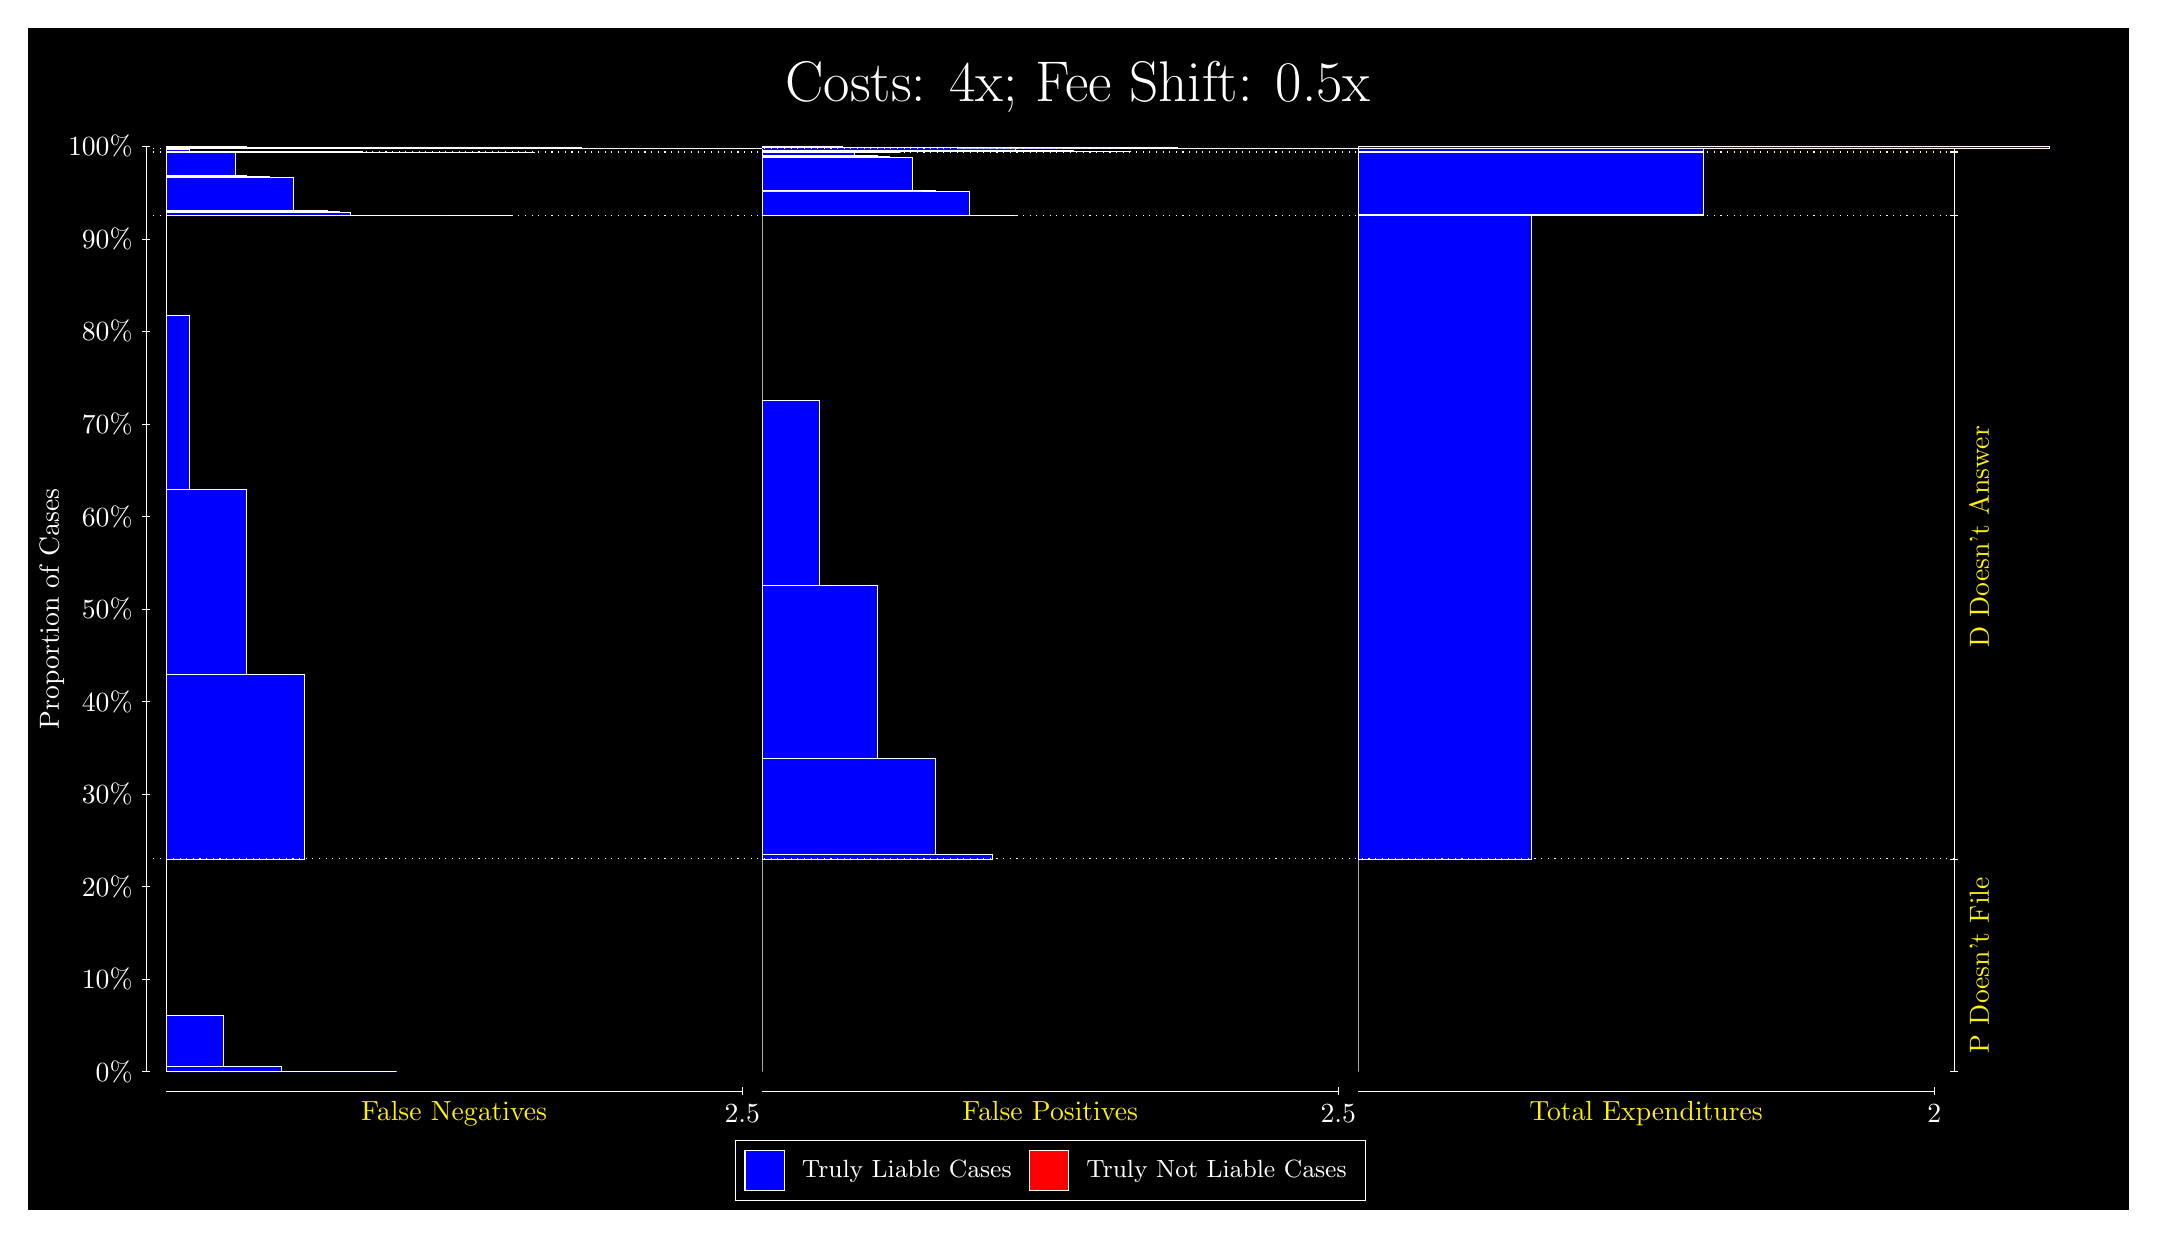
\begin{tikzpicture}
\draw[fill=black] (0,0) rectangle (26.667,15);
\draw[text=white] (0,13.5) rectangle (26.667,15) node[midway] {\huge Costs: 4x; Fee Shift: 0.5x};
\draw[white, very thin] (1.5,1.75) -- (1.5,13.5);
\node[rotate=90, text=white, anchor=center] at (0.3, 7.625) {Proportion of Cases};
\draw[white, very thin] (1.45,1.75) -- (1.55,1.75);
\node[text=white, anchor=east] at (1.45, 1.75) {0\%};
\draw[white, very thin] (1.45,2.925) -- (1.55,2.925);
\node[text=white, anchor=east] at (1.45, 2.925) {10\%};
\draw[white, very thin] (1.45,4.1) -- (1.55,4.1);
\node[text=white, anchor=east] at (1.45, 4.1) {20\%};
\draw[white, very thin] (1.45,5.275) -- (1.55,5.275);
\node[text=white, anchor=east] at (1.45, 5.275) {30\%};
\draw[white, very thin] (1.45,6.45) -- (1.55,6.45);
\node[text=white, anchor=east] at (1.45, 6.45) {40\%};
\draw[white, very thin] (1.45,7.625) -- (1.55,7.625);
\node[text=white, anchor=east] at (1.45, 7.625) {50\%};
\draw[white, very thin] (1.45,8.8) -- (1.55,8.8);
\node[text=white, anchor=east] at (1.45, 8.8) {60\%};
\draw[white, very thin] (1.45,9.975) -- (1.55,9.975);
\node[text=white, anchor=east] at (1.45, 9.975) {70\%};
\draw[white, very thin] (1.45,11.15) -- (1.55,11.15);
\node[text=white, anchor=east] at (1.45, 11.15) {80\%};
\draw[white, very thin] (1.45,12.325) -- (1.55,12.325);
\node[text=white, anchor=east] at (1.45, 12.325) {90\%};
\draw[white, very thin] (1.45,13.5) -- (1.55,13.5);
\node[text=white, anchor=east] at (1.45, 13.5) {100\%};

\draw[white, very thin] (24.457,1.75) -- (24.457,13.5);
\draw[white, very thin] (24.407,1.75) -- (24.507,1.75);
\node[anchor=west] at (24.407, 1.75) {};
\draw[white, very thin] (24.407,4.4507) -- (24.507,4.4507);
\node[anchor=west] at (24.407, 4.4507) {};
\draw[white, very thin] (24.407,12.626) -- (24.507,12.626);
\node[anchor=west] at (24.407, 12.626) {};
\draw[white, very thin] (24.407,13.425) -- (24.507,13.425);
\node[anchor=west] at (24.407, 13.425) {};
\draw[white, very thin] (24.407,13.437) -- (24.507,13.437);
\node[anchor=west] at (24.407, 13.437) {};
\draw[white, very thin] (24.407,13.473) -- (24.507,13.473);
\node[anchor=west] at (24.407, 13.473) {};
\draw[white, very thin] (24.407,13.5) -- (24.507,13.5);
\node[anchor=west] at (24.407, 13.5) {};

\draw[white, very thin, fill=blue] (1.75,1.75) rectangle (4.6775,1.75);
\draw[white, very thin, fill=blue] (1.75,1.75) rectangle (3.9457,1.7506);
\draw[white, very thin, fill=blue] (1.75,1.7506) rectangle (3.2138,1.818);
\draw[white, very thin, fill=blue] (1.75,1.818) rectangle (2.4819,2.4675);
\draw[white, very thin, fill=red] (1.75,2.4675) rectangle (1.75,2.4675);
\draw[white, very thin, fill=blue] (1.75,2.4675) rectangle (1.75,4.4507);
\draw[white, very thin, fill=blue] (1.75,4.4507) rectangle (3.5065,6.8006);
\draw[white, very thin, fill=blue] (1.75,6.8006) rectangle (2.7746,9.1494);
\draw[white, very thin, fill=blue] (1.75,9.1494) rectangle (2.0428,11.351);
\draw[white, very thin, fill=red] (1.75,11.351) rectangle (1.75,11.351);
\draw[white, very thin, fill=blue] (1.75,11.351) rectangle (1.75,12.626);
\draw[white, very thin, fill=blue] (1.75,12.626) rectangle (6.1413,12.626);
\draw[white, very thin, fill=blue] (1.75,12.626) rectangle (5.8486,12.626);
\draw[white, very thin, fill=blue] (1.75,12.626) rectangle (5.5558,12.626);
\draw[white, very thin, fill=blue] (1.75,12.626) rectangle (5.4094,12.626);
\draw[white, very thin, fill=blue] (1.75,12.626) rectangle (5.2631,12.626);
\draw[white, very thin, fill=blue] (1.75,12.626) rectangle (5.1167,12.626);
\draw[white, very thin, fill=blue] (1.75,12.626) rectangle (4.9703,12.626);
\draw[white, very thin, fill=blue] (1.75,12.626) rectangle (4.8239,12.626);
\draw[white, very thin, fill=blue] (1.75,12.626) rectangle (4.6775,12.627);
\draw[white, very thin, fill=blue] (1.75,12.627) rectangle (4.5312,12.627);
\draw[white, very thin, fill=blue] (1.75,12.627) rectangle (4.3848,12.627);
\draw[white, very thin, fill=blue] (1.75,12.627) rectangle (4.2384,12.627);
\draw[white, very thin, fill=blue] (1.75,12.627) rectangle (4.092,12.664);
\draw[white, very thin, fill=blue] (1.75,12.664) rectangle (3.9457,12.671);
\draw[white, very thin, fill=blue] (1.75,12.671) rectangle (3.7993,12.682);
\draw[white, very thin, fill=blue] (1.75,12.682) rectangle (3.6529,12.687);
\draw[white, very thin, fill=blue] (1.75,12.687) rectangle (3.5065,12.692);
\draw[white, very thin, fill=blue] (1.75,12.692) rectangle (3.3602,13.104);
\draw[white, very thin, fill=blue] (1.75,13.104) rectangle (3.2138,13.113);
\draw[white, very thin, fill=blue] (1.75,13.113) rectangle (3.0674,13.123);
\draw[white, very thin, fill=blue] (1.75,13.123) rectangle (2.921,13.124);
\draw[white, very thin, fill=blue] (1.75,13.124) rectangle (2.7746,13.126);
\draw[white, very thin, fill=blue] (1.75,13.126) rectangle (2.6283,13.425);
\draw[white, very thin, fill=blue] (1.75,13.425) rectangle (2.3355,13.425);
\draw[white, very thin, fill=blue] (1.75,13.425) rectangle (2.0428,13.425);
\draw[white, very thin, fill=red] (1.75,13.425) rectangle (1.75,13.425);
\draw[white, very thin, fill=blue] (1.75,13.425) rectangle (6.4341,13.425);
\draw[white, very thin, fill=blue] (1.75,13.425) rectangle (5.7022,13.425);
\draw[white, very thin, fill=blue] (1.75,13.425) rectangle (4.9703,13.427);
\draw[white, very thin, fill=blue] (1.75,13.427) rectangle (4.2384,13.437);
\draw[white, very thin, fill=blue] (1.75,13.437) rectangle (3.5065,13.437);
\draw[white, very thin, fill=red] (1.75,13.437) rectangle (1.75,13.437);
\draw[white, very thin, fill=blue] (1.75,13.437) rectangle (3.5065,13.437);
\draw[white, very thin, fill=blue] (1.75,13.437) rectangle (2.7746,13.438);
\draw[white, very thin, fill=blue] (1.75,13.438) rectangle (2.0428,13.459);
\draw[white, very thin, fill=red] (1.75,13.459) rectangle (1.75,13.459);
\draw[white, very thin, fill=blue] (1.75,13.459) rectangle (1.75,13.473);
\draw[white, very thin, fill=blue] (1.75,13.473) rectangle (9.9471,13.473);
\draw[white, very thin, fill=blue] (1.75,13.473) rectangle (9.2152,13.473);
\draw[white, very thin, fill=blue] (1.75,13.473) rectangle (8.4834,13.473);
\draw[white, very thin, fill=blue] (1.75,13.473) rectangle (7.7515,13.479);
\draw[white, very thin, fill=blue] (1.75,13.479) rectangle (7.0196,13.489);
\draw[white, very thin, fill=blue] (1.75,13.489) rectangle (6.2877,13.49);
\draw[white, very thin, fill=blue] (1.75,13.49) rectangle (5.7022,13.49);
\draw[white, very thin, fill=blue] (1.75,13.49) rectangle (4.9703,13.49);
\draw[white, very thin, fill=blue] (1.75,13.49) rectangle (4.2384,13.49);
\draw[white, very thin, fill=blue] (1.75,13.49) rectangle (3.5065,13.493);
\draw[white, very thin, fill=blue] (1.75,13.493) rectangle (2.7746,13.499);
\draw[white, very thin, fill=blue] (1.75,13.499) rectangle (2.0428,13.5);
\draw[white, very thin, fill=red] (1.75,13.5) rectangle (1.75,13.5);
\draw[white, very thin, fill=blue] (1.75,13.5) rectangle (1.75,13.5);
\draw[white, very thin, fill=red] (9.3189,1.75) rectangle (9.3189,1.75);
\draw[white, very thin, fill=blue] (9.3189,1.75) rectangle (9.3189,4.4507);
\draw[white, very thin, fill=red] (9.3189,4.4507) rectangle (12.246,4.4507);
\draw[white, very thin, fill=blue] (9.3189,4.4507) rectangle (12.246,4.5079);
\draw[white, very thin, fill=blue] (9.3189,4.5079) rectangle (11.515,5.7258);
\draw[white, very thin, fill=blue] (9.3189,5.7258) rectangle (10.783,7.9277);
\draw[white, very thin, fill=blue] (9.3189,7.9277) rectangle (10.051,10.276);
\draw[white, very thin, fill=blue] (9.3189,10.276) rectangle (9.3189,12.626);
\draw[white, very thin, fill=red] (9.3189,12.626) rectangle (12.539,12.626);
\draw[white, very thin, fill=blue] (9.3189,12.626) rectangle (12.539,12.626);
\draw[white, very thin, fill=red] (9.3189,12.626) rectangle (12.246,12.626);
\draw[white, very thin, fill=blue] (9.3189,12.626) rectangle (12.246,12.626);
\draw[white, very thin, fill=red] (9.3189,12.626) rectangle (11.954,12.626);
\draw[white, very thin, fill=blue] (9.3189,12.626) rectangle (11.954,12.925);
\draw[white, very thin, fill=blue] (9.3189,12.925) rectangle (11.807,12.927);
\draw[white, very thin, fill=red] (9.3189,12.927) rectangle (11.661,12.927);
\draw[white, very thin, fill=blue] (9.3189,12.927) rectangle (11.661,12.928);
\draw[white, very thin, fill=blue] (9.3189,12.928) rectangle (11.515,12.938);
\draw[white, very thin, fill=red] (9.3189,12.938) rectangle (11.368,12.938);
\draw[white, very thin, fill=blue] (9.3189,12.938) rectangle (11.368,12.948);
\draw[white, very thin, fill=blue] (9.3189,12.948) rectangle (11.222,13.359);
\draw[white, very thin, fill=blue] (9.3189,13.359) rectangle (11.075,13.364);
\draw[white, very thin, fill=blue] (9.3189,13.364) rectangle (10.929,13.369);
\draw[white, very thin, fill=blue] (9.3189,13.369) rectangle (10.783,13.38);
\draw[white, very thin, fill=blue] (9.3189,13.38) rectangle (10.636,13.387);
\draw[white, very thin, fill=blue] (9.3189,13.387) rectangle (10.49,13.424);
\draw[white, very thin, fill=blue] (9.3189,13.424) rectangle (10.344,13.424);
\draw[white, very thin, fill=blue] (9.3189,13.424) rectangle (10.197,13.425);
\draw[white, very thin, fill=blue] (9.3189,13.425) rectangle (10.051,13.425);
\draw[white, very thin, fill=blue] (9.3189,13.425) rectangle (9.9044,13.425);
\draw[white, very thin, fill=blue] (9.3189,13.425) rectangle (9.758,13.425);
\draw[white, very thin, fill=blue] (9.3189,13.425) rectangle (9.6116,13.425);
\draw[white, very thin, fill=blue] (9.3189,13.425) rectangle (9.4652,13.425);
\draw[white, very thin, fill=blue] (9.3189,13.425) rectangle (9.3189,13.425);
\draw[white, very thin, fill=red] (9.3189,13.425) rectangle (11.075,13.425);
\draw[white, very thin, fill=blue] (9.3189,13.425) rectangle (11.075,13.425);
\draw[white, very thin, fill=blue] (9.3189,13.425) rectangle (10.344,13.436);
\draw[white, very thin, fill=blue] (9.3189,13.436) rectangle (9.6116,13.437);
\draw[white, very thin, fill=blue] (9.3189,13.437) rectangle (9.3189,13.437);
\draw[white, very thin, fill=red] (9.3189,13.437) rectangle (14.003,13.437);
\draw[white, very thin, fill=blue] (9.3189,13.437) rectangle (14.003,13.437);
\draw[white, very thin, fill=blue] (9.3189,13.437) rectangle (13.271,13.451);
\draw[white, very thin, fill=blue] (9.3189,13.451) rectangle (12.539,13.473);
\draw[white, very thin, fill=blue] (9.3189,13.473) rectangle (11.807,13.473);
\draw[white, very thin, fill=blue] (9.3189,13.473) rectangle (11.075,13.473);
\draw[white, very thin, fill=red] (9.3189,13.473) rectangle (17.516,13.473);
\draw[white, very thin, fill=blue] (9.3189,13.473) rectangle (17.516,13.473);
\draw[white, very thin, fill=red] (9.3189,13.473) rectangle (16.784,13.473);
\draw[white, very thin, fill=blue] (9.3189,13.473) rectangle (16.784,13.473);
\draw[white, very thin, fill=red] (9.3189,13.473) rectangle (16.052,13.473);
\draw[white, very thin, fill=blue] (9.3189,13.473) rectangle (16.052,13.474);
\draw[white, very thin, fill=red] (9.3189,13.474) rectangle (15.32,13.474);
\draw[white, very thin, fill=blue] (9.3189,13.474) rectangle (15.32,13.48);
\draw[white, very thin, fill=blue] (9.3189,13.48) rectangle (14.588,13.483);
\draw[white, very thin, fill=blue] (9.3189,13.483) rectangle (13.857,13.483);
\draw[white, very thin, fill=blue] (9.3189,13.483) rectangle (13.125,13.483);
\draw[white, very thin, fill=blue] (9.3189,13.483) rectangle (12.393,13.483);
\draw[white, very thin, fill=red] (9.3189,13.483) rectangle (11.807,13.483);
\draw[white, very thin, fill=blue] (9.3189,13.483) rectangle (11.807,13.484);
\draw[white, very thin, fill=red] (9.3189,13.484) rectangle (11.075,13.484);
\draw[white, very thin, fill=blue] (9.3189,13.484) rectangle (11.075,13.494);
\draw[white, very thin, fill=blue] (9.3189,13.494) rectangle (10.344,13.5);
\draw[white, very thin, fill=blue] (9.3189,13.5) rectangle (9.6116,13.5);
\draw[white, very thin, fill=blue] (9.3189,13.5) rectangle (9.3189,13.5);
\draw[white, very thin, fill=red] (16.888,1.75) rectangle (16.888,1.75);
\draw[white, very thin, fill=blue] (16.888,1.75) rectangle (16.888,4.4507);
\draw[white, very thin, fill=red] (16.888,4.4507) rectangle (19.083,4.4507);
\draw[white, very thin, fill=blue] (16.888,4.4507) rectangle (19.083,12.626);
\draw[white, very thin, fill=red] (16.888,12.626) rectangle (21.279,12.626);
\draw[white, very thin, fill=blue] (16.888,12.626) rectangle (21.279,12.635);
\draw[white, very thin, fill=red] (16.888,12.635) rectangle (21.279,12.635);
\draw[white, very thin, fill=blue] (16.888,12.635) rectangle (21.279,13.425);
\draw[white, very thin, fill=red] (16.888,13.425) rectangle (21.279,13.425);
\draw[white, very thin, fill=blue] (16.888,13.425) rectangle (21.279,13.437);
\draw[white, very thin, fill=red] (16.888,13.437) rectangle (21.279,13.437);
\draw[white, very thin, fill=blue] (16.888,13.437) rectangle (21.279,13.473);
\draw[white, very thin, fill=red] (16.888,13.473) rectangle (25.67,13.473);
\draw[white, very thin, fill=blue] (16.888,13.473) rectangle (25.67,13.5);
\draw[white, dotted] (1.5,4.4507) -- (24.457,4.4507);
\draw[white, dotted] (1.5,12.626) -- (24.457,12.626);
\draw[white, dotted] (1.5,13.425) -- (24.457,13.425);
\draw[white, dotted] (1.5,13.437) -- (24.457,13.437);
\draw[white, dotted] (1.5,13.473) -- (24.457,13.473);
\draw[white, very thin] (1.75,1.5) -- (9.0689,1.5);
\node[text=yellow, anchor=north] at (5.4094, 1.5) {False Negatives};
\draw[white, very thin] (9.0689,1.45) -- (9.0689,1.55);
\node[text=white, anchor=north] at (9.0689, 1.45) {2.5};

\draw[white, very thin] (9.3189,1.5) -- (16.638,1.5);
\node[text=yellow, anchor=north] at (12.978, 1.5) {False Positives};
\draw[white, very thin] (16.638,1.45) -- (16.638,1.55);
\node[text=white, anchor=north] at (16.638, 1.45) {2.5};

\draw[white, very thin] (16.888,1.5) -- (24.207,1.5);
\node[text=yellow, anchor=north] at (20.547, 1.5) {Total Expenditures};
\draw[white, very thin] (24.207,1.45) -- (24.207,1.55);
\node[text=white, anchor=north] at (24.207, 1.45) {2};

\node[text=yellow, centered, rotate=90] at (24.777, 3.1004) {P Doesn't File};
\node[text=yellow, centered, rotate=90] at (24.777, 8.5386) {D Doesn't Answer};





\draw (12.978300999999998,1.5) node[draw=none] (baseCoordinate) {};
\begin{scope}[align=center]
        \matrix[scale=0.5, draw=white, below=0.5cm of baseCoordinate, nodes={draw}, column sep=0.1cm]{
            \node[rectangle, draw, minimum width=0.5cm, minimum height=0.5cm, fill=blue] {}; &
            \node[draw=none, font=\small, text=white] (B) {Truly Liable Cases}; &
            \node[rectangle, draw, minimum width=0.5cm, minimum height=0.5cm, fill=red] {}; &
            \node[draw=none, font=\small, text=white] (B) {Truly Not Liable Cases}; \\
            };
\end{scope}

\end{tikzpicture}
\end{document}